\begin{frame}{Scan Theory}
	\begin{itemize}
		\item Synonyms: prefix sum, cumulative sum or scan
		\item inclusive and exclusive version
		\item further specialization: segmented scan
	\end{itemize}
\end{frame} 
\begin{frame}{Inclusive Scan}
	\centering
	\vspace{-5pt}
	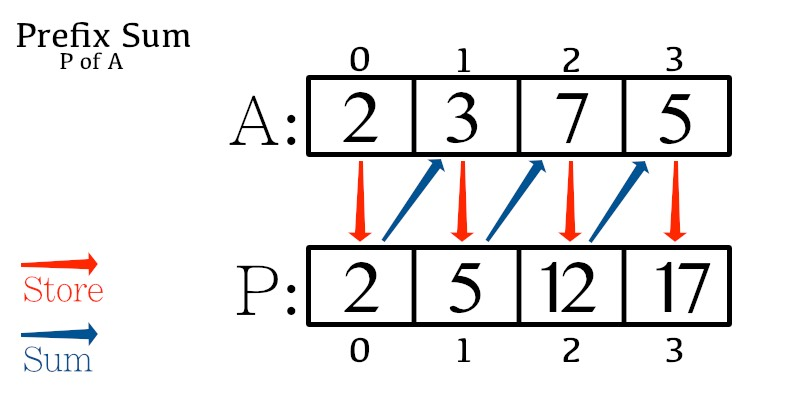
\includegraphics[width=0.90\textwidth]{"wiki/prefix-sum.jpg"}
	\tiny https://williamrjribeiro.com/?p=132
\end{frame}
\begin{frame}{inclusive vs. exclusive scan}
	\centering
	\vspace{-5pt}
	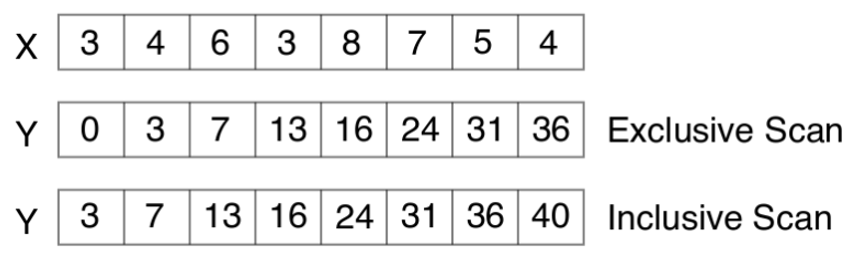
\includegraphics[width=0.90\textwidth]{"wiki/scans.png"}
	\tiny https://livebook.manning.com/book/parallel-and-high-performance-computing/chapter-5/v-11/
\end{frame}
\begin{frame}{segmented variant}
	\centering
	\vspace{-5pt}
	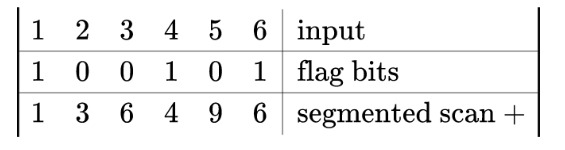
\includegraphics[width=0.90\textwidth]{"wiki/SegmentedScan.png"}
	\tiny https://en.wikipedia.org/wiki/Segmented\_scan

\end{frame}

